% Chaptre 1

\chapter{Approche suivie et solution proposée} % Main chapter title

\label{Chaptre4} % For referencing the chapter elsewhere, use \ref{Chapter1} 

Dans cette section nous ferons une présentation détaillée des solutions que nous avions proposées par rapport à nos missions.

%----------------------------------------------------------------------------------------

% Define some commands to keep the formatting separated from the content 
%\newcommand{\keyword}[1]{\textbf{#1}}
%\newcommand{\tabhead}[1]{\textbf{#1}}
%\newcommand{\code}[1]{\texttt{#1}}
%\newcommand{\file}[1]{\texttt{\bfseries#1}}
%\newcommand{\option}[1]{\texttt{\itshape#1}}
%----------------------------------------------------------------------------------------

\section{Méthodologie de travail: Scrum avec Agile}
\textbf{A compléter}
\section{Les différentes missions et solutions}
\subsection{Mission 1:Etude de faisabilité sur le déploiement d’une application Front-End dans un environnement AWS}
L’application frontend(web app flutter) de Gighamesh est hébergée sur Firebase, tandis que l’essentiel de
ses ressources se trouve dans le cloud d’Amazon. C’est dans le but d’unifier nos environnements cloud que
cette mission m’avait été confiée.
\subsubsection{Observations}
Les applications web Flutter sont  développées avec le langage de programmation Dart. Avant le déploiement d'une application Flutter un build est nécessaire, 
et le résultat de celui-ci est un ensembles des fichiers statiques( html, css, js, ...). Ce sont ces fichiers statiques qui sont déployés.
Pour résoudre  j’avais exploré deux possibilités:
\subsubsection{Solutions}
\subparagraph{Solution1: L’utilisation de S3 comme repos de d'hébergement}
La solution ici consiste à créer un repos S3, de le rendre public, afin de pouvoir accepter tous les trafics.
De configurer Code Pipeline pour les besoins de CI/CD avec Github, De configurer Cloudfront pour la
gestion du trafic et Route 54 pour le routage.
 \begin{figure}[!th]
            \centering
                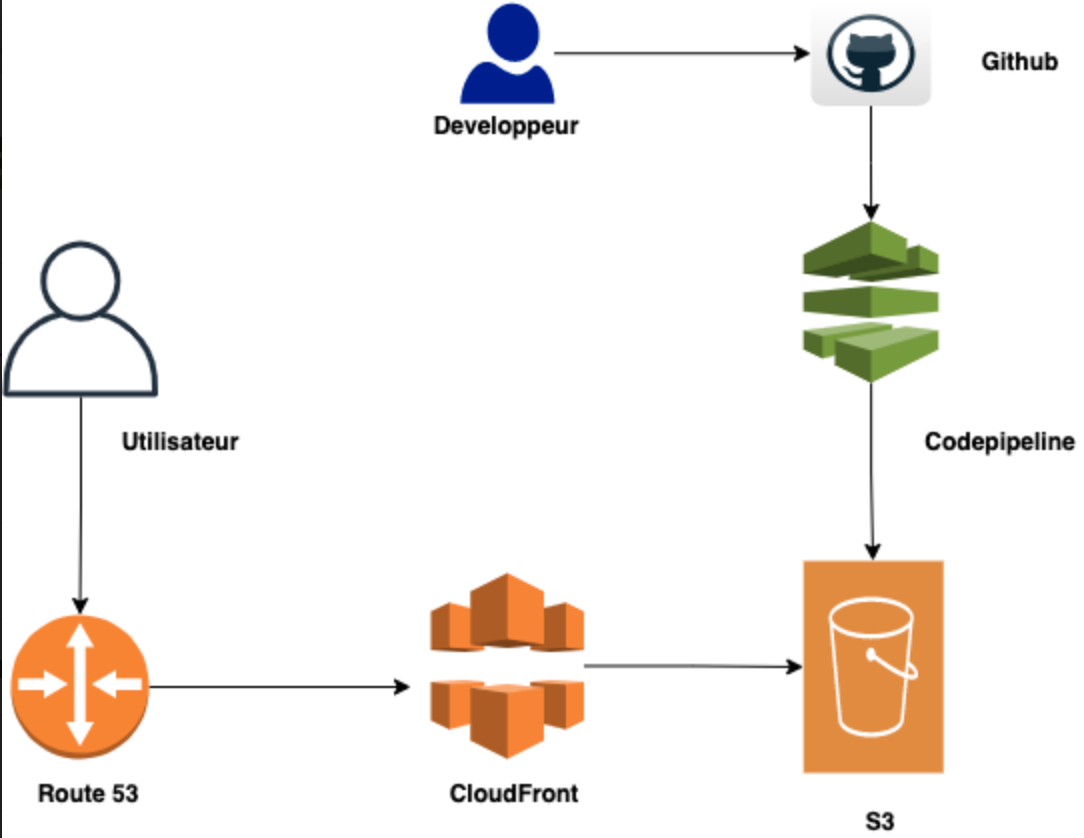
\includegraphics[width=0.8\textwidth]{Figures/S3}
	       \decoRule
		\caption[Solution à base de S3]{Solution à base de S3}
	\label{fig:S3}
	\end{figure}
%\newpage
\subparagraph{Solution2: L’utilisation d’Amplify comme comme repos d'hébergement}
Cette solution consiste à utiliser le service d’hébergement qu’offre Amplify et son système de CI/CD en
l’associant au système de versioning: Github. J'avais utilisé CloudFront pour la gestion du trafic et Route 54
pour le routage.
NB: C’est la solution 2 qui avait été retenue. Celle-ci est simple et plus adaptée.
 \begin{figure}[!th]
            \centering
                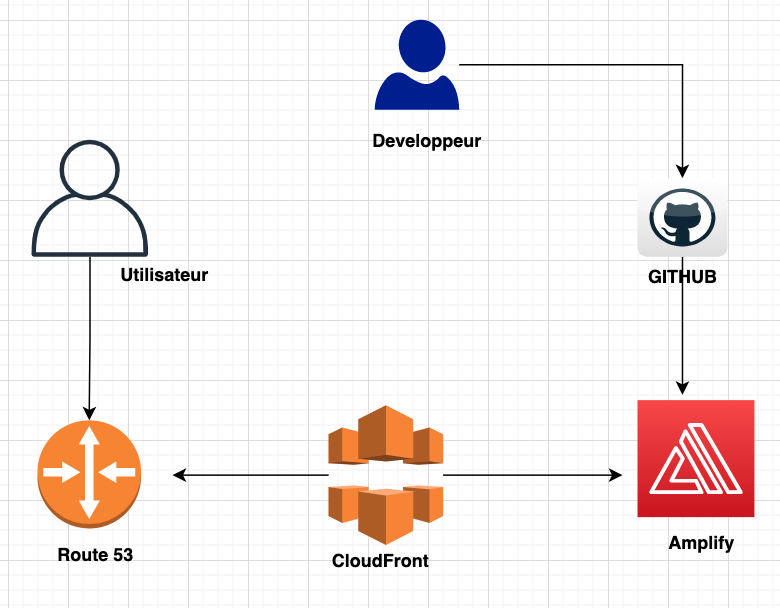
\includegraphics[width=0.8\textwidth]{Figures/amplify}
	       \decoRule
		\caption[Solution à base d'Amplify]{Solution à base d'Amplify}
	\label{fig:Amplify}
	\end{figure}
	
\subsection{Mission 2:Le déploiement et l’intégration du service web (Reflex) dans le parcours de spuscription}
La souscription au produit d’assurance Assurly est subdivisée en trois parcours: P1, P2, et P3. Un utilisateur ne peut se
retrouver que dans un seul parcours en fonction des données fournies. Si un utilisateur se retrouve dans le
parcours P3 un questionnaire plus complexe est nécessaire, c’est à cet instant qu’intervient Reflex.

\subsubsection{Solutions}
%Reflex est composé de trois modules de base: CEP pour frontend, DOCS pour la gestion des rapports et
%RAS qui constitue le cœur du système Reflex.
%La procédure de déploiement consiste mettre à jour le repos Github qui contient les fichiers nécessaires à la
%construction de notre container, à se connecter à notre EC2, à puller les fichiers du repos Github depuis un
%répertoire de notre EC2 puis à construire et déployer notre container avec la commande docker-compose.
\subsubsection{Pipeline de déploiement}
Quand nous recevons de notre partenaire des mises à jour des modules Reflex , nous les déployons(push) sur un repos Github. Notre repos Github est connecté à notre docker hub; ce qui déclenche automatiquement la construction et le déploiement(push) de l'image de notre conteneur sur docker hub. Pour déployer Reflex sur notre EC2: Il suffit soit de récupérer(pull) le contenu du repos Github puis construire l'image et déployer le conteneur ou de récupérer(pull) l'image de docker hub puis déployer le conteneur. La figure ci-dessous illustre le processus.  
 \begin{figure}[!th]
            \centering
                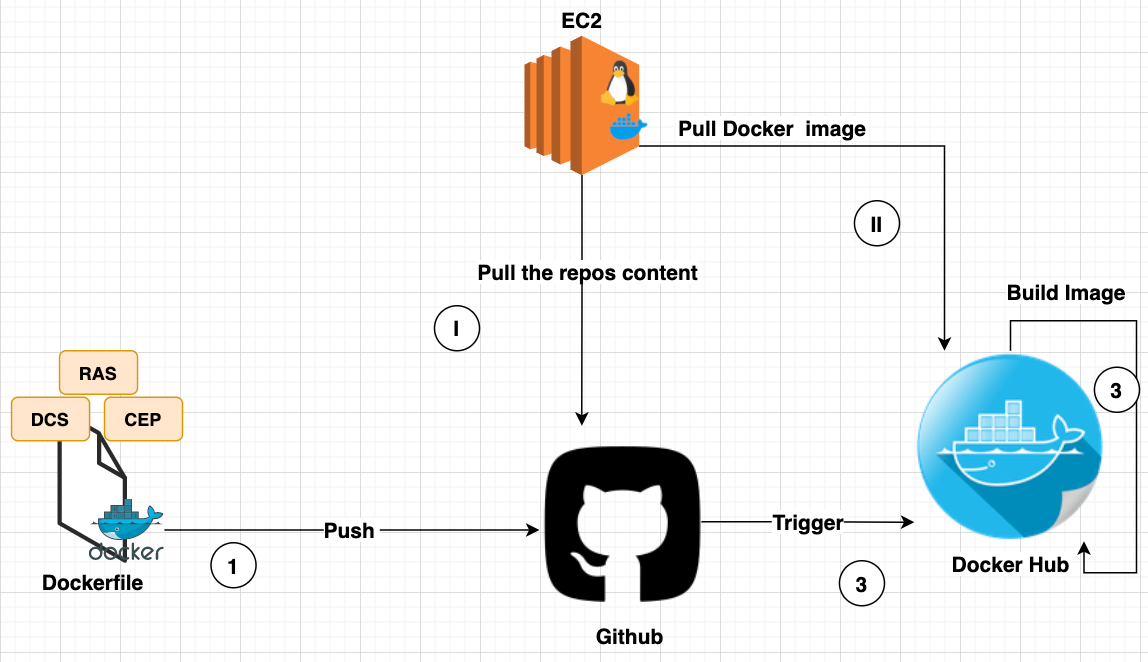
\includegraphics[width=0.8\textwidth]{Figures/pipeline1}
	       \decoRule
		\caption[Pipeline de déploiement de Reflex]{Pipeline de déploiement de Reflex}
	\label{fig:Pipeline de déploiement de Reflex}
\end{figure}

 \begin{figure}[!th]
            \centering
                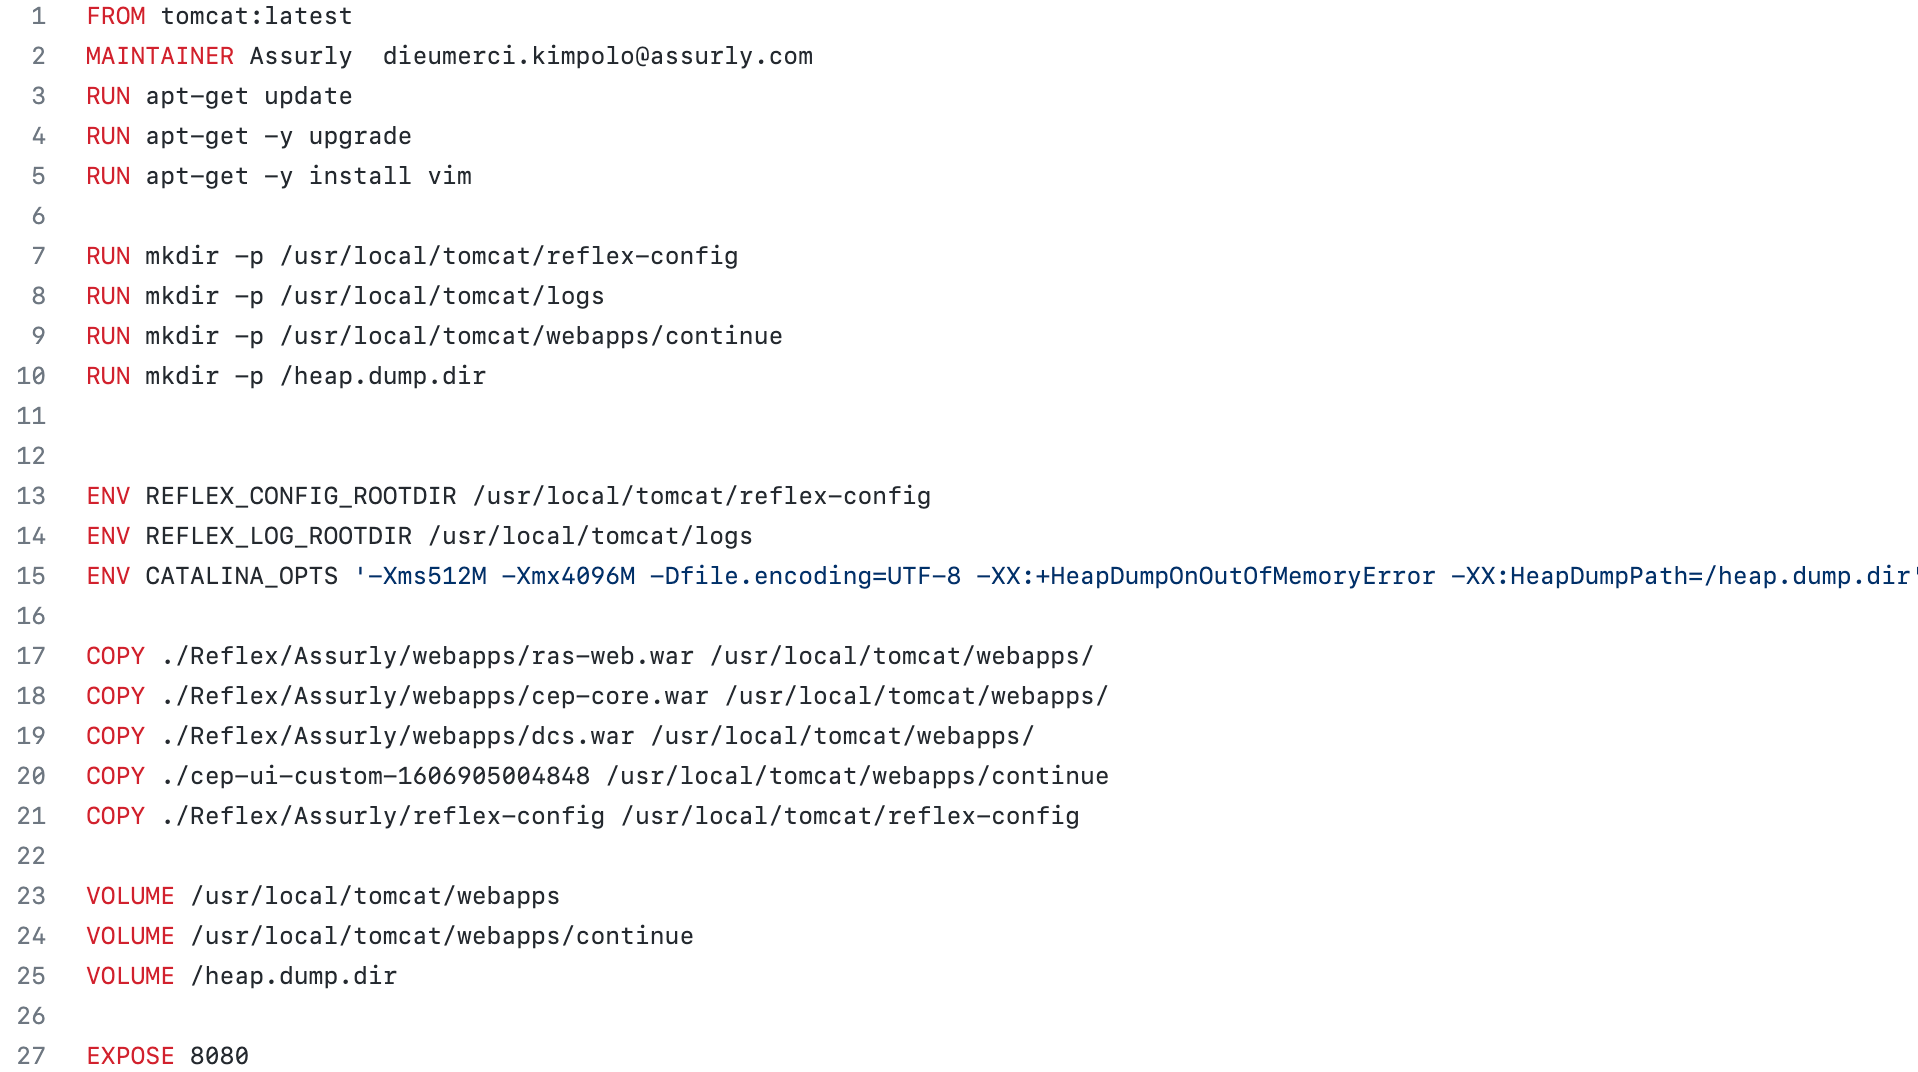
\includegraphics[width=0.8\textwidth]{Figures/dockerfile}
	       \decoRule
		\caption[Dockerfile de construction de l'image Reflex]{Dockerfile de construction de l'image Reflex}
	\label{fig:Dockerfile de construction de l'image Reflex}
\end{figure}

\subsubsection{Diagramme de séquence intégration}
L'intégration de Reflex sur l'application web est différente de celle sur l'application mobile.

\textbf{Cas de l'application web}
Notre application web est embarquée dans une Iframe, et l'intégration de Reflex passe par une initialisation des cookies. Il nous était impossible d'initialiser les cookies d'une autre domaine depuis l'Iframe de notre application web. Pour palier ce problème nous avons développé une application intermédiaire hébergée sur le même server web que le moteur Reflex. Les utilisateurs en P3 qui passe par notre application web sont redirigés  sur  l'application web intermédiaire, pour soumettre leur questionnaire Reflex et sont redirigés sur l'application web depart à la fin du processus. Le BACKEND sur le diagramme de séquences ci-dessous représente notre infrastructure dans l'environnement AWS.
 \begin{figure}[!th]
            \centering
                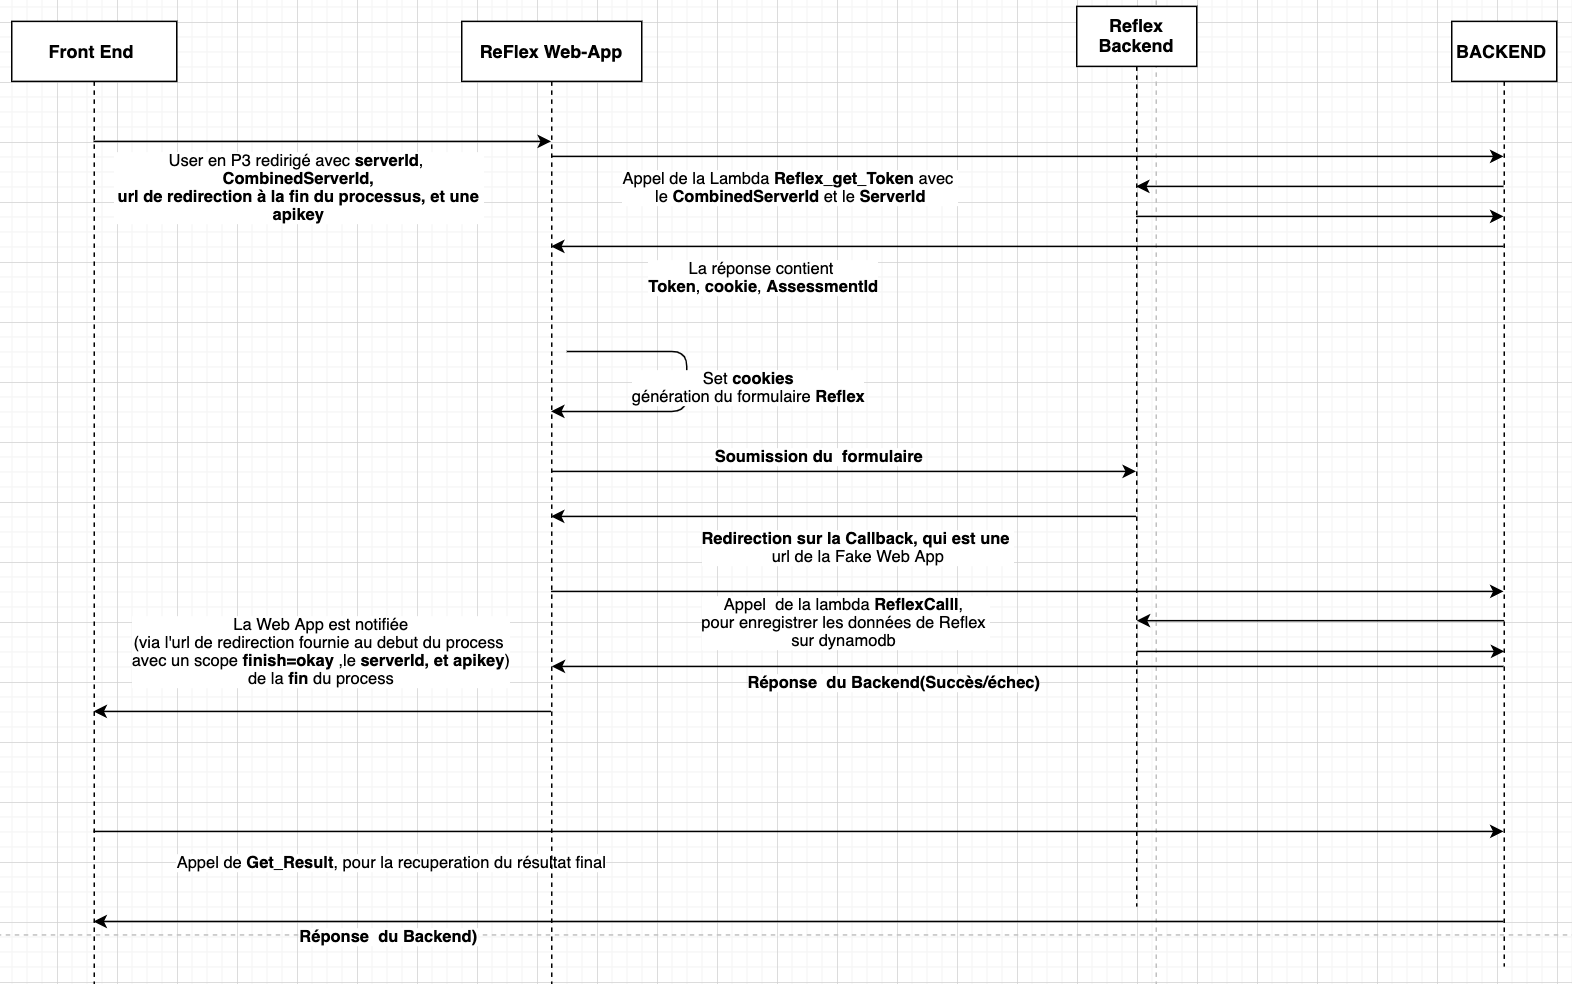
\includegraphics[width=0.8\textwidth]{Figures/reflexweb}
	       \decoRule
		\caption[Diagramme d'intégration de Reflex sur l'application web]{Diagramme d'intégration de Reflex sur l'application web}
	\label{fig:Diagramme d'intégration de Reflex sur l'application web}
\end{figure}

\subsection{Mission 3: (Sécurisation d’une API Rest développée avec la technologie Serveless d’AWS (Lambada + python))}
Pour sécuriser une API il faut prendre en compte deux aspects:
\begin{enumerate}
\item Les contrôles d'accès 
\item L'authentification et les autorisations
\end{enumerate}
Il n'ya pas de choix à faire entre les contrôles d'accès et le système d'authentification \& d'autorisation, ils sont complémentaires.
\subsubsection{Authentification et autorisations}
\textbf{Observations}
\begin{enumerate}
\item Dans l'environnement AWS c'est le service Cognito qui gère  les authentifications et les autorisations 
\item Cognito à la base ne peut supporter qu'un seul user pool (support de stockage des utilisateurs) sur une API
\item Nos utilisateurs sont stockés sur plusieurs users
\end{enumerate}

C'est Cognito que nous avons utilisé pour gérer les authentifications et les autorisations. Pour supporter plusieurs user pools sur nos API, nous avons développé un système d'autorisation 
personnalisé à base d'une Lambda. Dans notre implémentation nous avons explorer deux flows: l'implicit grant(en utilisant la web UI de Cognito) et password grant.
\textbf{Implicit grant}
 \begin{figure}[!th]
            \centering
                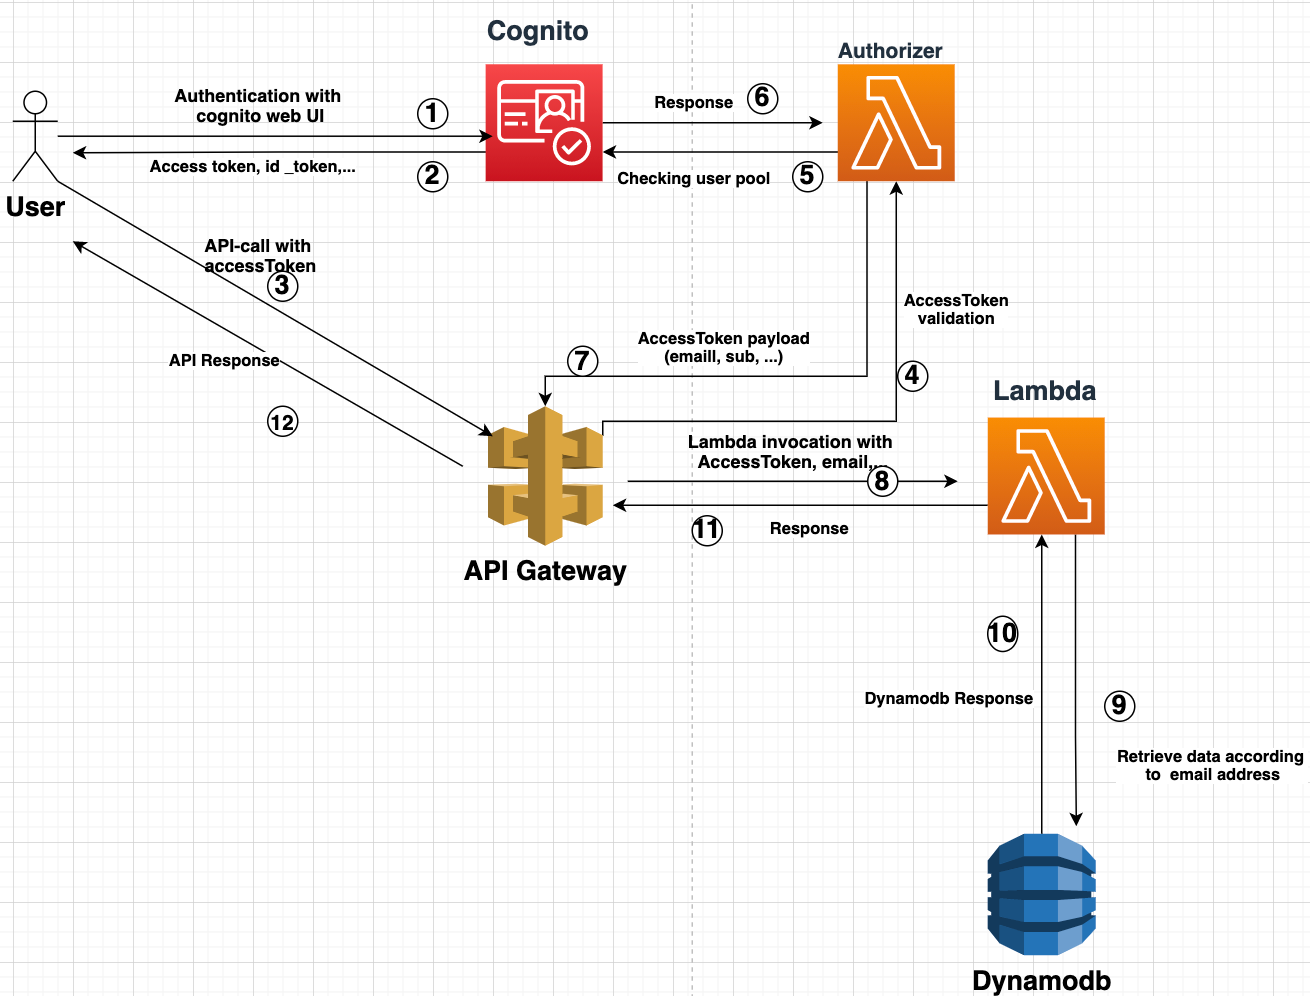
\includegraphics[width=0.8\textwidth]{Figures/securite}
	       \decoRule
		\caption[L'architecture du système de sécurité, Implicit grant]{L'architecture du système de sécurité, Implicit grant}
	\label{fig:L'architecture du système de sécurité, Implicit grant}
	\end{figure}
\textbf{Password grant}
 \begin{figure}[!th]
            \centering
                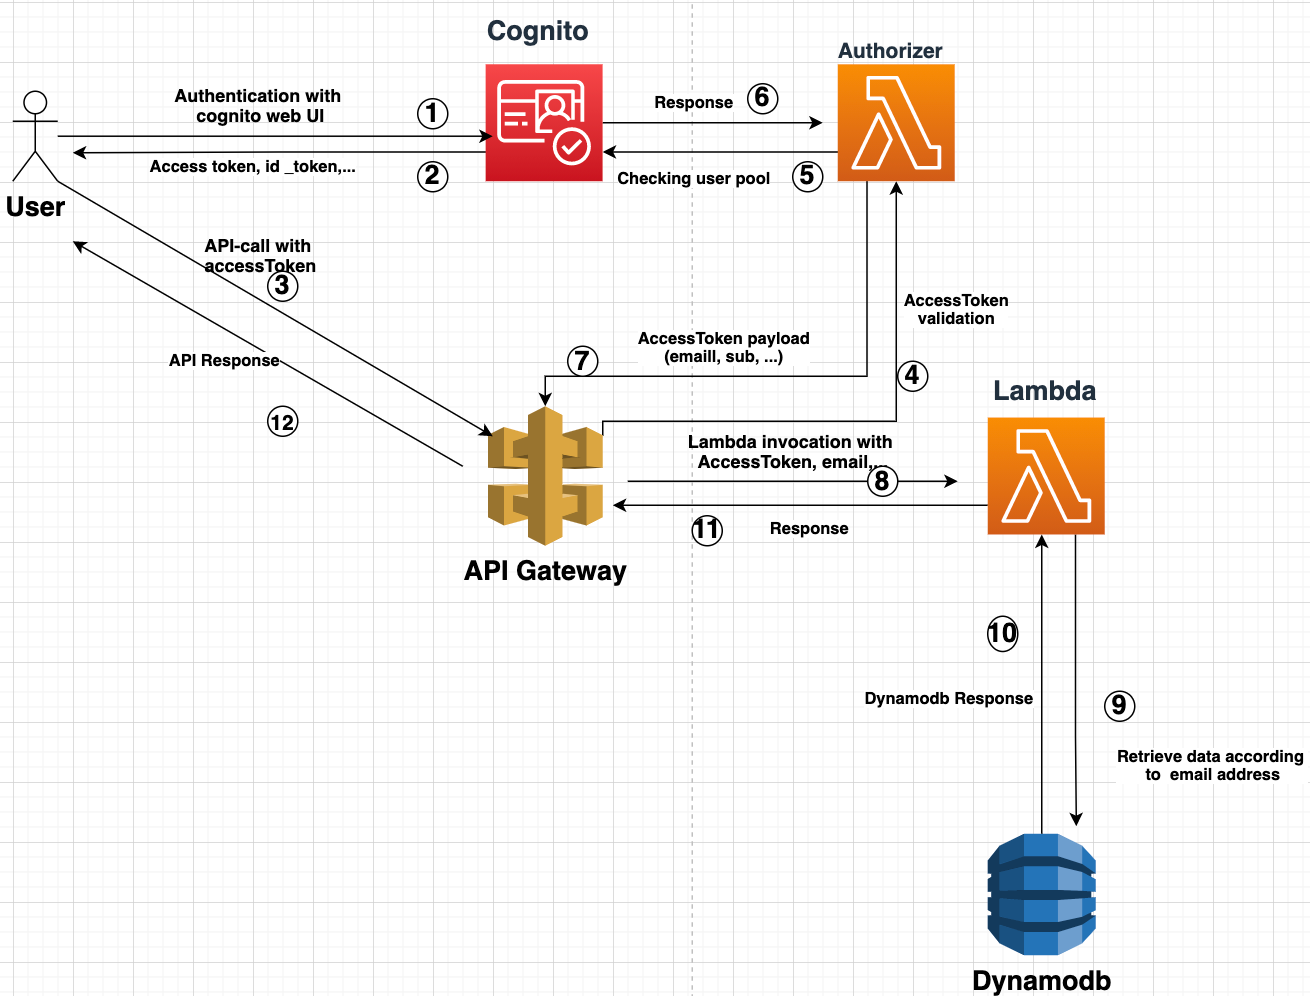
\includegraphics[width=0.8\textwidth]{Figures/securite}
	       \decoRule
		\caption[L'architecture du système de sécurité, Password grant]{L'architecture du système de sécurité, Password grant}
	\label{fig:L'architecture du système de sécurité, Password grant}
	\end{figure}
\newpage
\subsection{Mission 4(Mise en place d'un ETL d'intégration de données)}
Gigamesh disposait une quantité importantes des données stockées dans des fichiers txt; des données nécessaires pour effectuer des campagnes de marketing ciblées. Ma mission consistait à intégrer ces données dans une base de données sql pour pouvoir y effectuer facilement  des requêtes.

\subsubsection{Observations}
\begin{enumerate}
\item Tous les fichiers avaient la même structure
\item Le caractère | était utilisé comme séparateur des colonnes
\item Les libellés des colonnes étaient de fois des phrases
\item Les données n'étaient pas typées
\end{enumerate}
\subsubsection{Solution}
Pour résoudre le problème j'avais mise en place un \textbf{ETL}, qui récupère les données brutes(fichiers txt) de leur support de stockage, les transforme avec un \textbf{script Python} et les stocke dans base de données Mysql dans l'environnement AWS via le service Aurora. 

 \begin{figure}[!th]
            \centering
                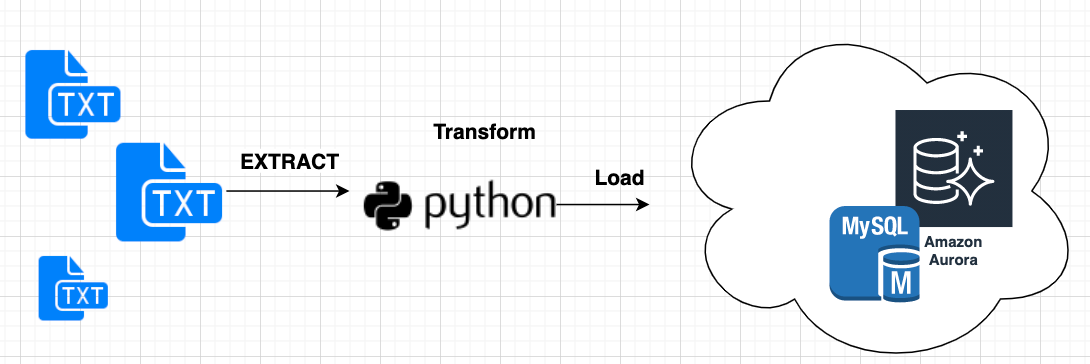
\includegraphics[width=0.8\textwidth]{Figures/etls}
	       \decoRule
		\caption[Etl d'intégration de données]{Etl d'intégration de données}
	\label{fig:etl}
	\end{figure}
La partie de transformation de mon ETL m'avait servi à la création de la table où sont stockées les données et à leur typage. 
